\everymath{\displaystyle}
\documentclass{beamer}
% \documentclass[handout]{beamer}

%\usepackage[pdftex]{color,graphicx}
\usepackage{amsmath,amssymb,amsfonts}

\mode<presentation>
{
  % \usetheme{Darmstadt}
  % \usetheme[hideothersubsections]{Hannover}
  % \usetheme[hideothersubsections]{Goettingen}
  \usetheme[hideothersubsections, right]{Berkeley}

  \usecolortheme{seahorse}
  % \usecolortheme{dolphin}
  \usecolortheme{rose}
  % \usecolortheme{orchid}

  \useinnertheme[shadow]{rounded}

  \setbeamercovered{transparent}
  % or whatever (possibly just delete it)
}

\mode<handout>{
  \setbeamercolor{background canvas}{bg=black!5}
  \usepackage{pgfpages}
  \pgfpagesuselayout{4 on 1}[a4paper,border shrink=5mm, landscape]
}

\usepackage[brazilian]{babel}
% or whatever

% \usepackage[latin1]{inputenc}
\usepackage[utf8]{inputenc}
% or whatever

\usepackage{times}
%\usepackage[T1]{fontenc}
% Or whatever. Note that the encoding and the font should match. If T1
% does not look nice, try deleting the line with the fontenc.


\title%[] % (optional, use only with long paper titles)
{Revisão e Resumo}

\subtitle
{} % (optional)

\author%[] % (optional, use only with lots of authors)
{Felipe Figueiredo}% \and S.~Another\inst{2}}
% - Use the \inst{?} command only if the authors have different
%   affiliation.

\institute[INTO] % (optional, but mostly needed)
{Instituto Nacional de Traumatologia e Ortopedia
}
  % \inst{1}%
  % Department of Computer Science\\
  % University of Somewhere
  % \and
  % \inst{2}%
  % Department of Theoretical Philosophy\\
  % University of Elsewhere}
% - Use the \inst command only if there are several affiliations.
% - Keep it simple, no one is interested in your street address.

\date%[] % (optional)
{}

% \subject{Talks}
% This is only inserted into the PDF information catalog. Can be left
% out. 



% If you have a file called "university-logo-filename.xxx", where xxx
% is a graphic format that can be processed by latex or pdflatex,
% resp., then you can add a logo as follows:

\pgfdeclareimage[height=1.6cm]{university-logo}{../logo}
\logo{\pgfuseimage{university-logo}}



% Delete this, if you do not want the table of contents to pop up at
% the beginning of each subsection:
\AtBeginSubsection[]
%\AtBeginSection[]
{
  \begin{frame}<beamer>{Sumário}
    \tableofcontents[currentsection,currentsubsection]
  \end{frame}
}


% If you wish to uncover everything in a step-wise fashion, uncomment
% the following command: 

\beamerdefaultoverlayspecification{<+->}


\begin{document}

\begin{frame}
  \titlepage
\end{frame}

\begin{frame}{Sumário}
  \tableofcontents
  % You might wish to add the option [pausesections]
\end{frame}


%% Template
% \section{}

% \subsection{}

% \begin{frame}{}
%   \begin{itemize}
%   \item 
%   \end{itemize}
% \end{frame}

% \begin{frame}
%   \begin{columns}
%     \begin{column}{5cm}
%     \end{column}
%     \begin{column}{5cm}
%     \end{column}
%   \end{columns}
% \end{frame}

% \begin{frame}{}
%   \includegraphics[height=0.4\textheight]{file1}
%   \includegraphics[height=0.4\textheight]{file2}
%   \includegraphics[height=0.4\textheight]{file3}
%   \begin{figure}
%     \caption{}
%   \end{figure}
% \end{frame}

% \begin{frame}{}
%   \begin{definition}
%   \end{definition}
%   \begin{example}
%   \end{example}
%   \begin{block}{Exercício}
%   \end{block}
% \end{frame}

\section{Revisão}

\begin{frame}{}
  \begin{itemize}
  \item 
  \end{itemize}
\end{frame}

\subsection{Revisão}

\begin{frame}{}
  \begin{itemize}
  \item 
  \end{itemize}
\end{frame}

\section{Resumo}

\begin{frame}{Definição}
  \begin{itemize}
  \item Mostra os aspectos principais do trabalho ou projeto
  \item linguagem técnica, sucinto
  \item curto
  \end{itemize}
\end{frame}

\subsection{Resumo}

\begin{frame}{Objetivos do resumo}
  \begin{itemize}
  \item Ajudar o leitor a decidir se ele deve ler o texto completo

%O leitor vai usar o abstract de artigos quando for fazer o levantamente bibliográfico.

  \item Ajudar o leitor a lembrar fatos importantes de um assunto

%Depois de ler vários artigos, pode ser difícil para o leitor se lembrar onde uma certa informação ou fato foi obtido, para fins de citação

  \item Ajudar o leitor a entender um texto difícil (pré-leitura
    sumária)

  \item Indexar artigos para fácil localização e referência

  \item Permitir que supervisores se mantenham atualizados na produção
    do lab
  \end{itemize}
\end{frame}

\begin{frame}{Tipos de resumo}
  \begin{itemize}
  \item Resumo descritivo
  \item Resumo estruturado (informativo)
  \end{itemize}
\end{frame}

\begin{frame}{Resumo descritivo}
  \begin{itemize}
  \item Descreve os principais tópicos do texto
  \item ``sumário em forma de parágrafo''
  \item não substitui a leitura do texto
  \end{itemize}
\end{frame}

\begin{frame}{Resumo descritivo}
  \begin{example}

    % \bigskip

    % \url{http://www.lter.alaska.edu/pubs/1997pr.html}

    We continue to document all major climatic variables in the
    uplands and floodplains at Bonanza Creek. In addition, we have
    documented the successional changes in microclimate in 9
    successional upland and floodplain stands at Bonanza Creek (BNZ)
    and in four elevational locations at Caribou-Poker Creek
    (CPCRW). A sun photometer is operated cooperatively with NASA to
    estimate high-latitude atmospheric extinction coefficients for
    remote-sensing images. Electronic data are collected monthly and
    loaded into a database which produces monthly summaries.  (...)

    % The data are checked for errors, documented, and placed on-line on
    % the BNZ Web page. Climate data for the entire state have been
    % summarized for the period of station records and krieged to
    % produce maps of climate zones for Alaska based on growing-season
    % and annual temperature and precipitation.
  \end{example}
  ``Bonanza Creek LTER [Long Term Ecological Research] 1997 Annual
  Progress Report''

\end{frame}

\begin{frame}{Resumo informativo}
  \begin{itemize}
  \item Inclui os detalhes essenciais do texto
  \item É suficiente para a decisão de ler ou não o texto completo
  \item Pode ser usado para mapear informações, fatos e dados
  \item Mais usado para artigos experimentais
  \end{itemize}
\end{frame}

\begin{frame}{Resumo informativo}
  Componentes típicos do resumo informativo
  \begin{itemize}
  \item Contexto e/ou motivação
  \item Objetivo, apresentação do problema
  \item Metodologia (para trabalhos experimentais)
  \item Principais resultados e descobertas
  \item Principais conclusões
  \end{itemize}
\end{frame}

\begin{frame}{Resumo informativo}
  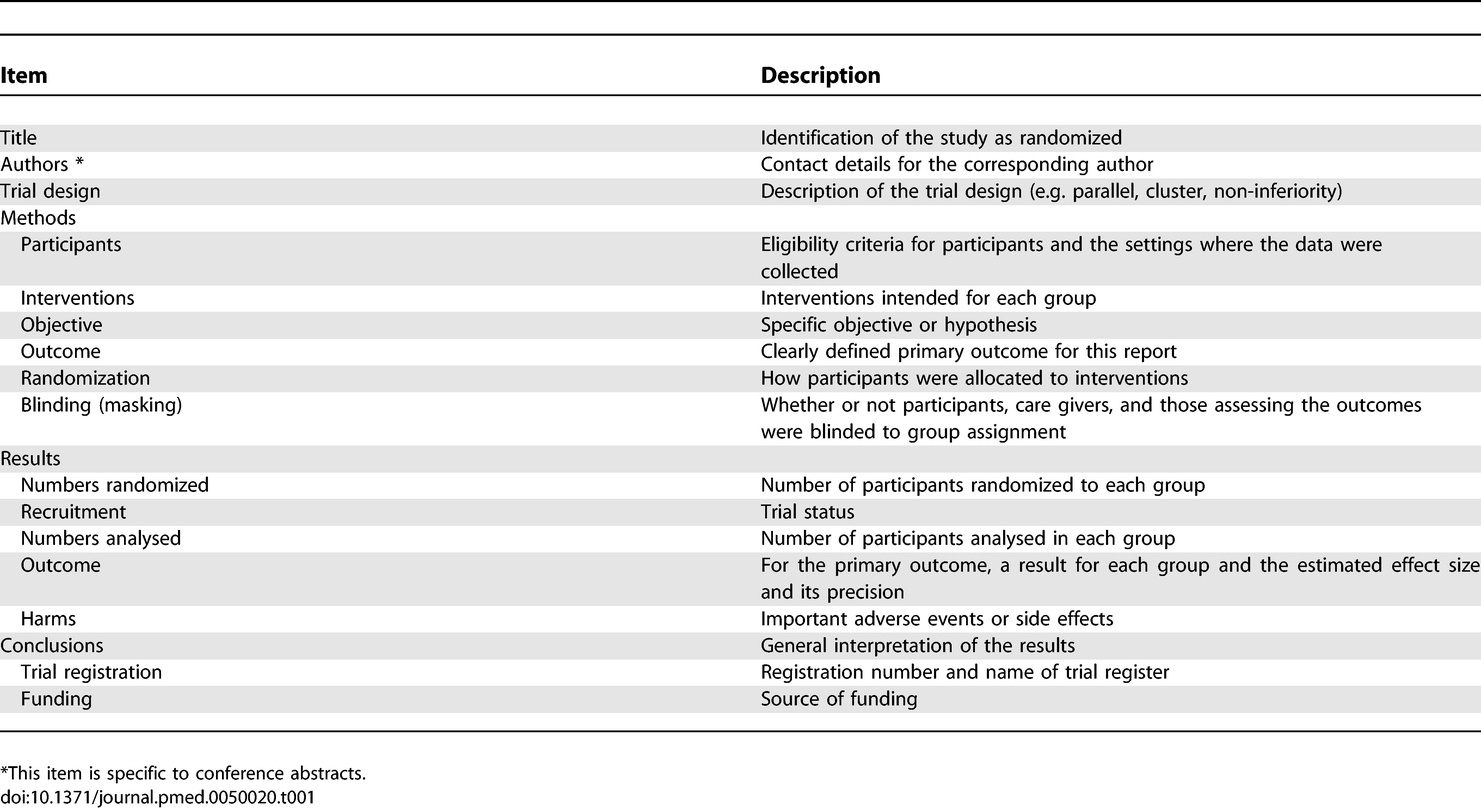
\includegraphics[height=0.8\textheight]{resumo_estruturado}
\end{frame}

\begin{frame}{Resumo informativo}
  \begin{example}

    % \bigskip

    Research reported by Daly, Miller, and their colleagues suggests
    that writing apprehension is related to a number of factors we do
    not yet fully understand. This study suggests that included among
    those factors should be the belief that writing ability is a
    gift. Giftedness, as it is referred to in the study, is roughly
    equivalent to the Romantic notion of original genius. Results from
    a survey of 247 postsecondary students enrolled in introductory
    writing courses at two institutions indicate that higher levels of
    belief in giftedness are correlated with higher levels of writing
    apprehension, (...) 

    % lower self-assessments of writing ability, lower levels of
    % confidence in achieving proficiency in certain writing activities
    % and genres, and lower self-assessments of prior experience with
    % writing instructors.  Significant differences in levels of belief
    % in giftedness were also found among students who differed in their
    % perceptions of the most important purpose for writing, with
    % students who identified "to express your own feelings about
    % something" as the most important purpose for writing having the
    % highest mean level of belief in giftedness. Although the validity
    % of the notion that writing ability is a special gift is not
    % directly addressed, the results suggest that belief in giftedness
    % may have deleterious effects on student writers.
  \end{example}
  ``Palmquist, M., \& Young, R. (1992). The Notion of Giftedness and
  Student Expectations About Writing. Written Communication, 9(1),
  137-168.''

\end{frame}

\end{document}
